\chapter{Alternatives}
\section{Representation of a Role Model as Individual}
\label{sec:A_representations}
	\subsection{Representation as Bit-string}
	The representation of individuals as bit-string is one of the simplest and is often mistakenly used in genetic algorithms\cite{Eiben}. A suggestion for a bit-string representation for a role model is derived from a combined user-role- (UA) and role-permission-matrix (PA). Figure \ref{fig:representation1} shows an example of a combined UA- and PA-Matrix and an according bit-string representation.
	
	\begin{figure}
		\centering
		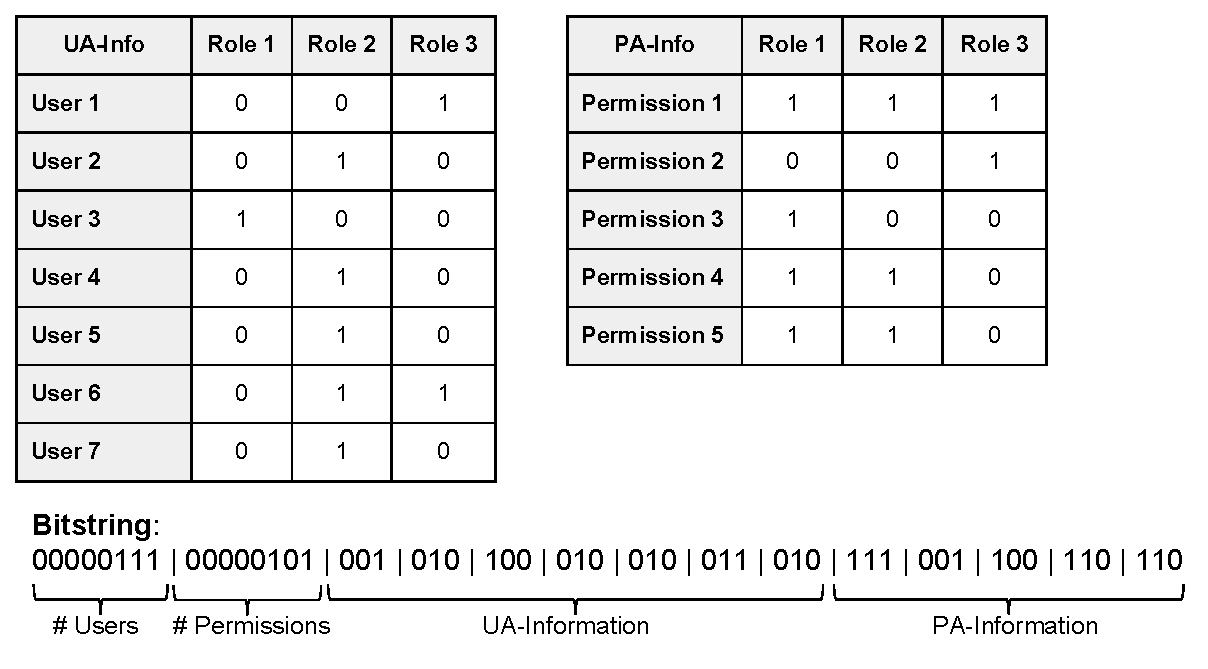
\includegraphics[scale=0.5]{BitstringRepresentation}
		\caption{\textit{Example of a UA- and PA-Matrix with its bit-string representation}}
		\label{fig:representation1}
	\end{figure}
	
	The motivation of this initial idea is that the mutation operator can be easily executed by just flipping a bit within the bit-string. The mutation is therefore adding or removing a user or permission from a role. For the decoding two leading 8-bit integers can represent the number of users and permission. However, the problem with this representation is that the number of roles needs to be pre-defined, such that the bit-string can be decoded again. Alternatively another leading 8-bit integer can represent the number of roles in the role model. But varying the number of roles demands adding or removing bits in the bit-string for each user-role- and role-permission relation. Furthermore the information that a user or a permission is not part of a role seems to unnecessarily lengthens the bit-string, which can consume a lot of space for high-dimensional UA- and PA-Matrices.

	\subsection{Representation as Multi-chromosomal Objects}
	In Saenko \& Kotenko\cite{saenko2012design} two different representations are introduced, which are briefly described in section \ref{sec:relatedWork3}. With the first representation the authors suggest a multi-chromosomal representation where the number of roles becomes part of the search. An example can be seen in figure \ref{fig:representation2}. A drawback of this representation are unnecessary genes (roles) like the unnecessary information in the bit-string representation. Another disadvantage of the representation are complex crossover operations\cite{saenko2012design}.
	
	\begin{figure}[H]
		\centering
		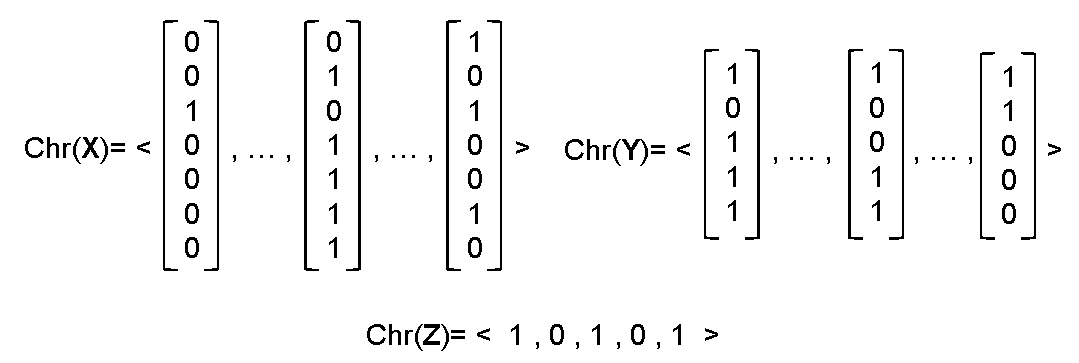
\includegraphics[scale=0.5]{ComplexRepresentation1}
		\caption{Example of a multi-chromosomal representation. Chromosome X represents the UA-Informationa and Chromosome Y the PA-Information. Chromosome Z determines if a role is active or passive. The columns in all chromosomes are consistent to roles. In this example roles 1, 3 and 5 are active.}
		\label{fig:representation2}
	\end{figure}